\documentclass[a4paper,10pt]{article}
\usepackage[utf8]{inputenc}
\usepackage{amsmath}
\usepackage{graphicx}
\usepackage[spanish]{babel} 
% author definitions
\def\bforce{{\boldsymbol{F}}}
\def\btorque{{\boldsymbol{M}}}
\def\bB{{\boldsymbol{B}}}
\def\bb{{\boldsymbol{b}}}
\def\bbp{{\boldsymbol{b}_{\rm p}}}
\def\br{{\boldsymbol{r}}}
\def\ba{{\boldsymbol{a}}}
\def\bA{{\boldsymbol{A}}}
\def\bAp{\boldsymbol{A}_{\rm p}}
\def\bk{{\boldsymbol{k}}}
\def\bJ{{\boldsymbol{J}}}
\def\bu{{\boldsymbol{u}}}
\def\bE{{\boldsymbol{E}}}
\def\rot{\boldsymbol{\nabla \times}}
\def\grad{\boldsymbol{\nabla}}
\def\div{\boldsymbol{\nabla \cdot}}
\def\dt#1{\frac{\partial #1}{\partial t}}
\def\dx#1{\frac{\partial #1}{\partial x}}
\def\dy#1{\frac{\partial #1}{\partial y}}
\def\dz#1{\frac{\partial #1}{\partial z}}
\def\f#1#2#3#4{{f}_{#1,#2,#3}^{(#4)}}
\def\bF#1{\boldsymbol{F}(#1)}
\def\bFd#1{\boldsymbol{F_D}(#1)}
\def\bx{B_x}
\def\by{B_y}
\def\bz{B_z}
\def\bxobs{B_x^{\rm (obs)}}
\def\byobs{B_y^{\rm (obs)}}
\def\bzobs{B_z^{\rm (obs)}}
\def\lapl{\nabla^2}
\def\lapl2D{\nabla^2_{xy}}
\def\bBobs{{\boldsymbol{B}}^{\rm (obs)}}
\def\nota#1{{\bf NOTA: #1}}
\def\eq#1{Ecuación (\ref{#1})}
\def\eqs#1#2{Ecuaciones (\ref{#1}) y (\ref{#2})}
\def\bBp{\boldsymbol{B}_{\rm p}}
\def\bBj{\boldsymbol{B}_{\rm J}}
\def\bBps{\boldsymbol{B}_{\rm p,s}}
\def\bBjs{\boldsymbol{B}_{\rm J,s}}
\def\bBpns{\boldsymbol{B}_{\rm p,ns}}
\def\bBjns{\boldsymbol{B}_{\rm J,ns}}
\def\dn#1{\frac{\partial #1}{\partial {\hat n}}}
\def\jperp{\bJ_\perp}
%opening
\title{Notas para la implementación NLFFF}
\author{Federico A. Nuevo}

\begin{document}

\maketitle

\begin{abstract}
Estas notas describen la implementación de un modelo de campo libre de fuerzas no líneal (NLFFF). 
\end{abstract}

\section{Introducción}

El problema se puede dividir en tres etapas:
\begin{enumerate}
 \item preprocesamiento (PP) de magnetogramas vectoriales fotosféricos.
 \item extrapolación coronal libre de fuerzas no líneal del anterior a partir del método magnetofriccional (Valori et al.; 2005, 2007)
 \item visualización y análisis del campo magnético. Esta etapa incluye el cálculo de energía, la helicidad y el análisis de la topología magnética (puntos nulos, capas cuasiseparatrices, etc).
\end{enumerate}

El campo magnético NLFFF cumple las ecuaciones:

\begin{equation}
 \rot \bB = \alpha (\br) \bB \,, \label{nlff}
\end{equation}
\begin{equation}
 \div \bB = 0 \label{div0} \,,
\end{equation}
sujeto a la condición de contorno:
\begin{equation}
\bB(x,y,z=0) = \bBobs(x,y) \label{ccfot} \,,
\end{equation}
donde $\bBobs$ es el campo magnético medido en la fotósfera extraido del magnetograma vectorial PP.

Para obtener la ecuación que cumple $\alpha$ se toma la divergencia de la \eq{nlff} y usando la \eq{div0} obtenemos:
\begin{equation}
( \bB \cdot \grad) \alpha = 0 \,.
\end{equation}
Esta significa que $\alpha$ es constante a lo largo de las líneas de campo. Combinando las \eqs{nlff}{ccfot}, la condición de contorno que cumple $\alpha$ en la fotósfera está dada por:
\begin{equation}
 \alpha (x,y,z=0) = \frac{\partial_x{\byobs}-\partial_y{\bxobs}}{\bzobs}\,.
\end{equation}
Esta evidencia la necesidad de magnetogramas vectoriales para condicionar modelos no lineales. Sin embargo, esta no es la mejor forma de plantear el problema, ya que el cálculo numérico de las derivadas introduce errores significativos. En particular en regiones donde $B_z$ es pequeño los errores involucrados aumentan considerablemente. La condición de contorno para $\alpha$ se debe aplicar solamente a una de las dos polaridades de campo en el magnetograma ($B_z>0$ ó $B_z<0$). El método magnetofriccional no requiere calcular $\alpha$ en la fotósfera, ni en la corona, utilizandose exclusivamente. el campo $\bBobs$ como condición de contorno. 


\section{Preprocesamiento}

El campo magnético fotosférico no es consistente con la condición libre de fuerzas. Para ver esto es conveniente calcular las fuerza magnética $\bforce$ sobre la caja de cálculo (Fuhrmann et al. 2007):
\begin{equation}
 F_x = -\frac{1}{\mu_0}\int_{\rm mgm} B_xB_z \,dx dy \,,
\end{equation}
\begin{equation}
 F_y = -\frac{1}{\mu_0}\int_{\rm mgm} B_yB_z \,dx dy \,,
\end{equation}
\begin{equation}
 F_z = \frac{1}{2\mu_0}\int_{\rm mgm}(B_x^2 + B_y^2 - B_z^2) \,dx dy \,.
\end{equation}
Las integrales en estas ecuaciones se realizan sobre la superficie matemática del magnetograma. Para deducir estas expresiones a partir de la fuerza de Lorentz (magnética) se usa el tensor de Maxwell $T_{i,j}=\frac{1}{\mu_0}\left(B_iB_j - \frac{1}{2}\delta_{ij}B^2 \right)$. El tensor de Maxwell debe integrarse en las seis fronteras de la caja pero como el campo decrece rapidamente en la corona las integrales sobre las fronteras laterales y superior pueden despreciarse. Así, queda solamente una integral sobre la frontera de abajo, que coincide con la superficie del magnetograma vectorial.

De forma similar el torque o momento de las fuerzas magnético $\btorque$ puede expresarse como (Fuhrmann et al. 2007):
\begin{equation}
 M_x= \frac{1}{2\mu_0} \int_{\rm mgm} y (B_x^2 + B_y^2 - B_z^2)\, dx dy \,,
\end{equation}
\begin{equation}
 M_y= \frac{1}{2\mu_0} \int_{\rm mgm} x (-B_x^2 - B_y^2 + B_z^2)\, dx dy \,,
\end{equation}
\begin{equation}
 M_z = \frac{1}{\mu_0}\int_{\rm mgm} (yB_xB_z - xB_y B_z )\, dx dy \,.
\end{equation}
De esta forma se puede verificar que cualquier magnetograma vectorial fotosférico tendrá valores no nulos de fuerza y torque. Lo que es inconsistente con la condición libre de fuerzas.

El objetivo del PP es modificar el campo medido por el magnetograma de manera que se minimizen las componentes de la fuerza y el torque sobre la caja de cálculo, logrando obtener una condición de contorno más consistente con la condición libre de fuerzas. Otro objetivo del PP es suavizar (regularizar) el magnetograma, es decir, reducir las irregularidades de pequeña escala del mismo. El suavizado del magnetograma compite con la reducción de la fuerza y el torque en el proceso de minimización.
Para una discusión detallada sobre el PP ver Fuhrmann et al. (2007) y Fuhrmann et al. (2011).
%
Existen dos métodos de PP. Uno desarrollado por Wiegelmann (PPTW, de ahora en más) y otro por Fuhrmann (PPMF, de ahora en más), utilizado por Valori.

\subsection{PP de Wiegelmann (PPTW)}

Wiegelmann et al. (2006) desarrollaron una rutina de PP en la que implementan lo explicado arriba.  Para ello plantean un funcional del campo magnetico $\bB$ con cuatro términos:
\begin{equation}
 L^{(\rm TW)}(\bB)=\mu_1L_1(\bB)+\mu_2L_2(\bB)+\mu_3L_3(\bB)+\mu_4L_4(\bB) \,,
\end{equation}
donde los coeficientes $\mu_i$ ($i=1,..., 4$) dan distinto peso a los diferentes términos del funcional.

El primer y segundo térmimo minimizan la fuerza y el torque magnético, respectivamente:
\begin{equation}
 L_1 = \left(\sum_P \bx\bz \right)^2+\left(\sum_P \by\bz \right)^2 + \left(\sum_P (\bx^2 + \by^2 - \bz^2)  \right)^2 \,,
 \label{L1}
\end{equation}
\begin{equation}
 L_2 = \left(\sum_P y(\bx^2 + \by^2 - \bz^2)  \right)^2 + \left(\sum_P x(-\bx^2 - \by^2 + \bz^2)  \right)^2 + \left(\sum_P (y\bx\bz - x\by\bz)  \right)^2 \,,
 \label{L2}
\end{equation}
donde las integrales se aproximan por sumatorias sobre los puntos de grilla $P$ del magnetograma (notar que falta el factor $\Delta x \Delta y$). 

El término de regularización que adoptan es
\begin{equation}
L_4 = \sum_P \left[ \left(\lapl2D \bx\right)^2 +\left(\lapl2D \by\right)^2 + \left(\lapl2D \bz\right)^2\right] \,,
\end{equation}
donde $\lapl2D = \partial^2_{xx}+\partial^2_{yy}$. De ahora en más lo llamaremos $L_4^{\rm TW}$ porque el PP de Fuhrmann usa otra técnica de regularización que involucra otra forma para este término del funcional.

El tercer término es:
\begin{equation}
 L_3 = \sum_P \left[(\bx - \bxobs)^2 + (\by - \byobs)^2 + (\bz - \bzobs)^2    \right] \,,
\end{equation}
donde $\bBobs$ es el campo magnético obtenido del magnetograma vectorial fotosférico. Este término penaliza apartamientos muy pronunciados respecto de las mediciones derivadas del magnetograma.


\subsection{PP de Fuhrmann (PPMF)}

La técnica de PPMF (Fuhrmann et al. 2007) consiste en minimizar el siguiente funcional: 

\begin{equation}
 L^{(\rm MF)}(\bB)=\mu'_1\frac{L_1(\bB)}{N_{L_1}}+\mu'_2\frac{L_2(\bB)}{N_{L_2}}+\mu'_4\frac{L^{(\rm MF)}_4(\bB)}{N^{(\rm MF)}_{L_4}} \,,
\end{equation}
donde los $\mu'_i$ ($i=1,2,4$) son los factores de peso del funcional.
$L_1$ y $L_2$ están dados por las \eqs{L1}{L2}. Es decir, son los mismos términos del funcional del PPTW, solamente que están adimensionalizados por las constantes: 
\begin{equation}
 N_{L_1} = \left[\sum_P |\bBobs|^2 \right]^2 \,,
\end{equation}
\begin{equation}
 N_{L_2} = \left[\sum_P \sqrt{x^2+y^2}|\bBobs|^2 \right]^2 \,. 
\end{equation}

El término de regularización adoptado en el PPMF es: 
\begin{equation}
 L^{(\rm MF)}_4 = \sum_{i=x,y,z}\,\sum_P \left\{ M_n \left[ B_i (x-nh,y-nh),...,B_i(x,y),...,B_i (x+nh,y+nh)\right]-B_i(x,y)\right\}^2 \,,
\end{equation}
donde $n$ es un número entero positivo y $M_n$ es la mediana de una ventana rectangular con $(2n+1)^2$ puntos de grilla centrada alrededor de $(x,y)$. Este método se denomina \emph{Windowed-median technique}. Obviamente, en los bordes del magnetograma no se puede aplicar este método. En esos puntos no se modifican los valores de campo y se espera que los mismos sean pequeños o nulos. Este subfuncional se adimensionaliza por
\begin{equation}
 N_{L^{(\rm MF)}_4}= L^{(\rm MF)}_4 (\bBobs) \,.
\end{equation}

Es importante notar que el PPMF, a diferencia del PPTW, no utiliza el subfuncional $L_3$ que provee una medida global de la diferencia entre el magnetograma original y el modificado por el PP. 

En vez de aplicar un subfuncional de ese estilo, el PPMF impone bordes prescriptos localmente en cada punto de grilla al proceso de optimización, los cuales no deben sobrepasarse en el mismo. En otras palabras, en el PPMF la minimización del funcional $L$ se realiza de forma que el campo no pueda variar respecto al campo observado más allá de cierto rango definido por las incertezas instrumentales.
 

\subsection{implementación numérica}

el códido de PP está escrito en lenguaje FORTRAN 90 ({\tt pp\_simann.f90}). Este código tiene basicamente dos entradas:
\begin{itemize}
 \item El magnetograma vectorial en formato FORTRAN 77 ({\tt mgm.dat}).
 \item un archivo de parámetros iniciales de nombre {\tt pp\_par.f}
\end{itemize}

Para preparar estas dos entradas, compilar el código y correrlo se utiliza un código auxiliar en lenguaje IDL ({\tt pp\_sharp.pro}). 

El código {\tt pp\_sharp.pro} lee el magnetograma vectorial usando la rutina {\tt read\_sdo} del SolarSoft. Busca los pixeles cuyo valor corresponden a NaNs y ceros. En dichos pixeles reemplaza los NaNs por ceros y los ceros por el valor medio de sus ocho pixeles vecinos.
%
Luego, el magnetograma es rebineado a la resolución deseada ($N_x$, $N_y$). 
%
Además, graba el magnetograma vectorial en formato FORTRAN usando la rutina {\tt openw} con flag {\tt /f77\_unformatted} y escribe en el archivo {\tt pp\_par.f}  los errores relativos y absolutos del campo magnético, la resolución del magnetograma ($N_x$, $N_y$) y los rangos de los ejes.

Finalmente el código se compila usando un makefile. En este paso surgió el primer problema. El código se debe compilar con el compilador de FORTRAN desarrollado por INTEL llamado ifortran. El mismo no es de acceso libre, por lo que tuve que conseguir una versión pirata. Las versiones crackeadas que conseguí eran lo suficientemente viejas para ser incompatibles con UBUNTU 12 o más recientes. Para lograr hacer funcionar el ifortran tuve que instalar una Virtual Machine con DEBIAN 5.  
%
Además logré compilar el código de PP con el compilador de FORTRAN de GNU (gfortran).
%
Usando ifortran el código es considerablemente más rápido pero gfortran es de acceso libre y no requiere piratearlo.\\

Para compilar con ifortran en el makefile debe estar seteado:\\

FC=ifort y
OPT=-O2 -r8  -parallel -openmp \\

Para compilar con gfortran: \\

FC=gfortran y
OPT=-ffree-line-length-0 -fdefault-real-8


\section{Extrapolación magnetofriccional (MF)}
\label{mafex_sec}

Una vez preprocesado el magnetograma fotosférico se procede a realizar la extrapolación coronal libre de fuerza del mismo. La extrapolación consiste en resolver las \eqs{nlff}{div0} usando como condición de contorno inferior la \eq{ccfot} (previo PP). Para realizar la misma se utiliza el método \emph{magnetofriccional}. Este método considera un campo magnético inicial, cuya componente normal cumple la condición de contorno fotosférica, que es evolucionado mediante un conjunto de ecuaciones magnetohidrodinámicas (MHD)  a un campo libre de fuerza. La evolución MHD del campo magnético es ficticia y solo es relevante el estado final obtenido. 

Las ecuaciones MHD que describen la evolución del campo magnético son
\begin{equation}
\rho \left[\dt{\bu}+(\bu \cdot \nabla)\bu\right] = -\nabla p + {\bJ}\times {\bB} + \bFd{\bu} \,,
\label{euler}
\end{equation}
\begin{equation}
\bE +  {\bu}\times {\bB} = \eta \bJ \,,
\label{ohm}
\end{equation}
\begin{equation}
 \dt{\bB} = -\rot \bE \,,
 \label{faraday}
\end{equation}
\begin{equation}
 \mu_0 \bJ = \rot \bB  \,,
\label{rotor}
\end{equation}
donde $\bFd{\bu}= -\nu\bu$ es una fuerza disipativa ficticia que sirve para que el campo relaje a un equilibrio libre de fuerzas. $\nu = B^2/\mu$ es una viscosidad numérica con $\mu=\mu(t)$ un parámetro que cambia en el tiempo, cuyo valor es (Valori et al., 2007)
\begin{equation}
 \mu = \mu_0 \frac{c_c \, c_y}{{\rm max}\left\{{\frac{\Delta x|\bJ \times \bB|}{\mu_0 B^2}}\right\}} \frac{{\Delta x}^2}{\Delta t} \,,
\end{equation}
donde $c_c$ y $c_y$ son constantes adimensionales menores a la unidad. $\Delta x$ y $\Delta t$ son los pasos de discretización espacial y temporal, respectivamente. Esta elección de la viscosidad numérica garantiza que se cumpla la condición CFL y de esta forma se logra obtener la estabilidad numérica del método durante la evolución temporal. 

En la \eq{euler} se desprecia el término inertivo y el gradiende de presión, este último debido a la condición $\beta \ll 1$. De esta forma obtenemos
\begin{equation}
 \nu {\bu}= {\bJ} \times {\bB} \,.
\label{frictional}
\end{equation}

De la \eq{ohm} podemos despejar el campo electrico y reemplazando en la \eq{faraday} obtenemos
\begin{equation}
\dt{\bB} = \rot (\bu \times \bB) -\rot(\eta \bJ) \,,
\label{induction}
\end{equation}
donde $\eta$ es una resistividad numérica y en la gran mayoría de las aplicaciones se elige $\eta=0$. 

Reemplazando en la \eq{induction} el valor de $\bu$ despejado de la \eq{frictional} y de $\bJ$ despejado de la \eq{rotor} obtenemos 
\begin{equation}
 \dt{\bB} = \frac{\mu}{\mu_0} \rot \left(\frac{[({ \rot \bB}) \times {\bB}] \times \bB}{B^2}\right) + C_L \grad (\div \bB) \,.
 \label{evolB}
\end{equation}
donde se agregó el término $ C_L \grad (\div \bB)$ para difundir efectos numéricos de  divergencias no nulas. $C_L=c_L {\Delta x}^2/\Delta t$, donde $c_L$ es una constante adimensional menor a uno. Esta elección de $c_L$ permite que se cumpla la condición CFL a todo tiempo.  

Dado un campo magnético inicial y una condición de contorno fotosférica, la \eq{evolB} determina la evolución temporal del campo magnético y su convergencia a un equilibrio libre de fuerza a tiempos largos. 
%
Las derivadas espaciales se calculan usando un esquema de diferencias finitas (FD) centrado de cuarto orden (Valori et al., 2007) y la evolución se realiza usando un esquema de integración temporal de Runge-Kutta-Chebyshev (Valori et al. 2010).
%
La condición inicial coincide en la base con la componente normal del magnetograma, pero no con las componentes tangenciales. Esto último inyecta una fuerza de Lorentz en el sistema y luego, debido a la fuerza disipativa, relaja a un equilibrio. Como la velocidad es proporcional a la fuerza de Lorentz segun la \eq{frictional}, al disiparse la velocidad el campo converge a un equilibrio libre de fuerza. Este esquema es denominado \emph{stress-and-relax method}.

Mas allá del escenario MHD propuesto, el método es una extrapolación magnética pura. Por lo tanto la velocidad de plasma que aparece en la \eq{frictional} es ficticia y solo es un medio para evolucionar el campo inicial (usualmente potencial o libre de fuerzas líneal) a un NLFFF. En la siguiente Sección describo aspectos técnicos de la implementación NLFFF en base al método magnetofriccional desarrollada por Valori. Algunos de estos aspectos no se encuentran presentes en los \emph{papers}.

\subsection{Implementación numérica}
Para obtener un modelo NLFFF a partir de un magnetograma vectorial se utiliza una grilla uniforme. La grilla en el plano $xy$ coincide con la grilla del magnetograma preprocesado (con resolución $\Delta x=\Delta y$ y tamaño $N_x \times N_y$). El número de puntos de grilla en el eje $z$  se define en función de la altura de la caja $L$ como $N_z=L/\Delta z$ donde $\Delta z = \Delta x= \Delta y$. El código tiene una opción para trabajar con una grilla no uniforme en z pero no la he explorado todavía. 

La grilla posee dos capas de celdas fantasmas en las condiciones de contorno laterales y superior y una capa de celdas fantasmas debajo de la fotósfera. Para una explicación detallada sobre la condiciones exigidas en estas capas de celdas fantasmas leer Valori et al. (2007).

Para obtener un modelo NLFFF a partir de un magnetograma vectorial se utiliza un esquema de grillado multiple (\emph{multigridding-scheme}).
%
El mismo consiste en hacer sucesivas extrapolaciones en distintas grillas 
pasando de menor a mayor resolución para obtener el modelo NLFFF deseado.

Inicialmente, se calcula el modelo en una grilla de resolución $N_x/4\times Ny/4 \times Nz/4$. Para ello se hace un congrid del magnetograma a la resolución reducida. Luego, se calcula como condición inicial un modelo potencial ($\bB=-\nabla \Phi$) que satisface $\bzobs$ en la fotósfera (pero no $\bxobs$ ni $\byobs$) usando el método de la función de Green (Sakurai 1982)
\begin{equation}
 \Phi (x,y,z) = \int dx'dy'\frac{\bzobs(x',y')}{\sqrt{(x-x')^2+(y-y')^2+z^2}} \,.
\end{equation}

Una vez obtenido el modelo NLFFF en la grilla de resolución $N_x/4\times Ny/4 \times Nz/4$ se interpola a una grilla de resolución intermedia de $N_x/2\times Ny/2 \times Nz/2$ y se usa este como condición inicial para una segunda extrapolación. Obtenida esta, se repite el procedimiento para obtener un modelo NLFFF en la resolución final ($N_x\times Ny\times Nz$). Entonces, para obtener un modelo NLFFF basado en un dado magnetograma se deben hacer 3 corridas sucesivas del código magnetofriccional. 

El código de extrapolación magnetofriccional esta escrito en lenguaje FORTRAN y se llama  {\tt chod.f}. En realidad se usa una versión ``condensada'' escrita en lenguaje PERL ({\tt chod.t}) que se lleva a lenguaje FORTRAN durante el proceso de compilación. Para preparar la condición inicial y la condición de contorno se utiliza un código de lenguaje IDL llamado {\tt mafex.pro} que se ejecuta a partir de un script de nombre {\tt launch\_mafex.idl}. 

Cabe agregar que desarrollé un programa que adapta la salida del modelo NLFFF a las suite de códigos de visualización desarrollados por Cristina y Pascal para su modelo líneal. Cómo ejemplo, la Figura \ref{ej} muestra una visualización de la líneas de campo del modelo NLFFF obtenido para la región activa (AR) 11836 (2013-09-03 UT 03:36) usando este suite de códigos.

\begin{figure}
\begin{center}
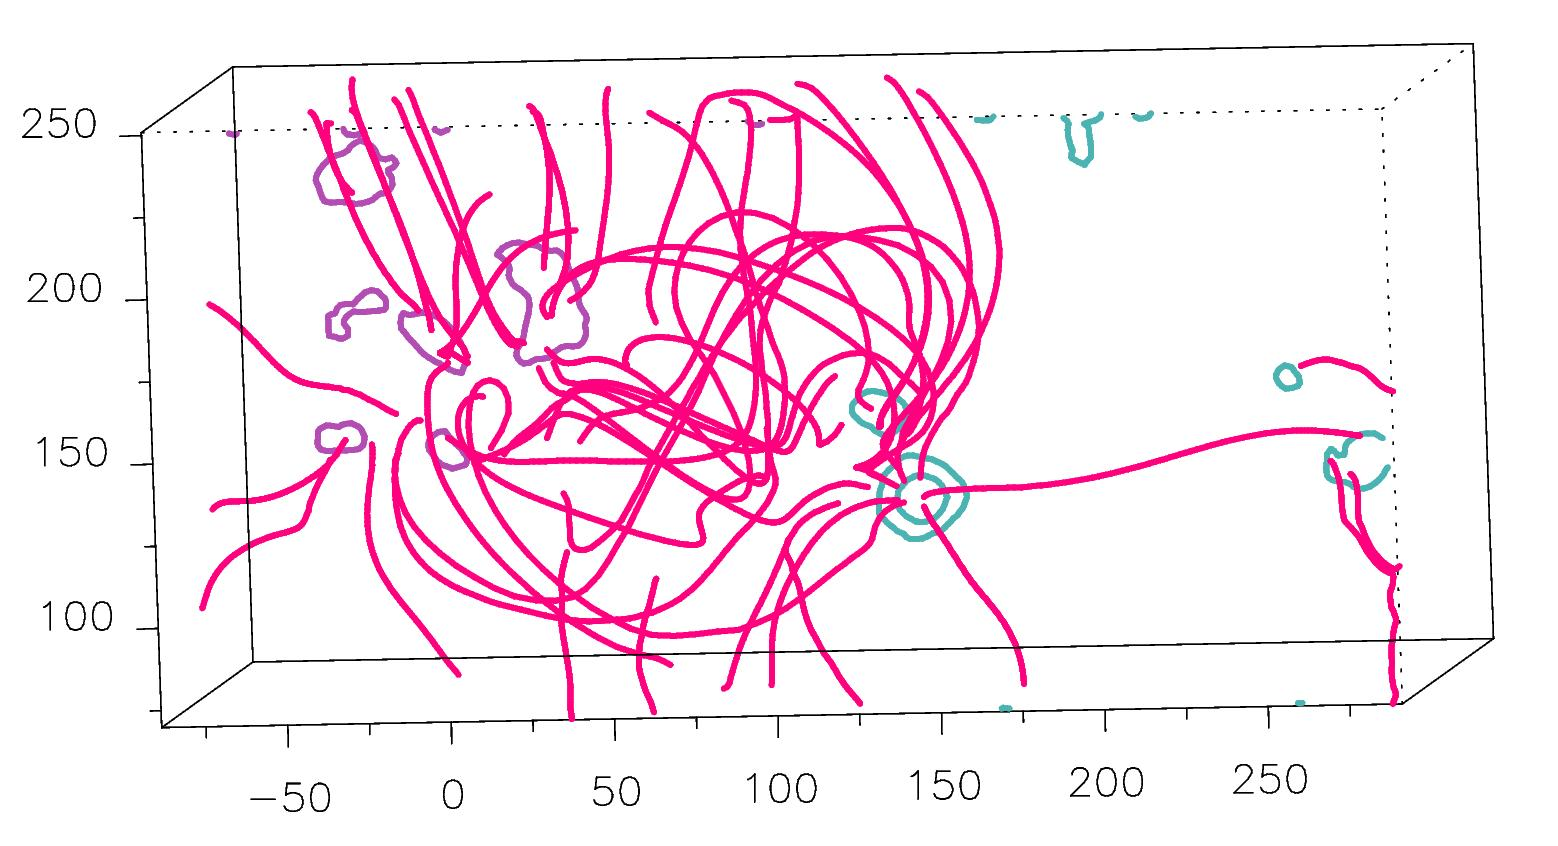
\includegraphics[width=0.75\textwidth]{fig/nlfff_test.jpg}
\end{center}
\caption{visualización de líneas de campo para el modelo NLFFF de la AR 11836 (2013-09-03 UT 03:36).}
%\vspace{-0.03\textwidth}
 \label{ej}
\end{figure}



\section{Cálculo de cantidades físicas}

Hay una suite de códigos de Gherardo que permiten cálcular cantidades físicas como energía magnética y helicidad dado un modelo NLFFF. Considero que también es importante aprender a usar estos códigos para poder analizar las extrapolaciones magnéticas realizadas. Para ello se debe usar el script {\tt ex\_analysis.idl} (adaptado a mi computadora con nombre {\tt comandos\_ex\_analysis.pro}) que ejecuta el código {\tt ex\_analysis.pro} (en el directorio .../macros/) que a su vez ejecuta el código {\tt thomson.pro} (en el directorio .../macros/thomson/). El código thomson tiene una subrutina {\tt solve\_poisson} que prepara el código en lenguaje FORTRAN {\tt poisson.f90}. Este código se compila con un makefile en la VM (donde está instalado el ifortran) y es el que invoca a la rutina {\tt mkl\_poisson.f90} perteneciente a la libreria MKL. A su vez {\tt thomson.pro} llama al programa {\tt helicity\_af.pro} que es el encargado de calcular la helicidad.

\subsection{Campo potencial de refencia}
\label{pot}

Tanto para el cálculo de la helicidad relativa como para el cálculo de la energía magnética usando el teorema de Thompson en necesario calcular previamente un campo magnético potencial ($\bBp = \nabla \Phi$) cuya componente normal en las fronteras de la caja coincidan con el campo obtenido en la Sección \ref{mafex_sec}. El potencial $\Phi$ cumple entonces la ecuación de Laplace
\begin{equation}
 \nabla^2 \Phi = 0 \,,
\end{equation}
sujeta a la condición de contorno de Neumann
\begin{equation}
\dn{\Phi} \rvert_{\partial V}  = (\bB \cdot {\hat n}) \rvert_{\partial V} \,.
\end{equation}
Para calcular $\Phi$ se utiliza el código {\tt mkl\_poisson.f90} de la libreria MKL.

\subsection{Helicidad magnética relativa}
\label{helicity_sec}

La helicidad magnética relativa la campo potencial $\bBp$ se define (Finn \& Antonsen, 1985):
\begin{equation}
 H = \int_V \, (\bA + \bAp) \cdot (\bB - \bBp) \,dV \,,
\end{equation}
donde $\bA$ y $\bAp$ son los potenciales vector de $\bB$ y $\bBp$, respectivamente. El volumen $V$ de la caja de cálculo esta dado por $[x_1; x_2] \times [y_1; y_2] \times [0; L]$.

La helicidad puede descomponerse en tres contribuciones 
\begin{equation}
 H = H_{\rm B} - H_{\rm P} + H_{\rm mix} \,, 
\end{equation}
donde:
\begin{equation}
 H_{\rm B} = \int_{V} \, \bA \cdot \bB \, dV \,,
\end{equation}
\begin{equation}
 H_{\rm P} = \int_{V} \, \bAp \cdot \bBp \,dV \,,
\end{equation}
\begin{equation}
 H_{\rm mix} = \int_{V} \, (\bAp \cdot \bB - \bA \cdot \bBp) \,dV \,.
\end{equation}

Para calcular los potenciales vectores se utiliza el siguiente gauge:
\begin{equation}
 \bA \cdot \hat z = \bAp \cdot \hat z = 0 \,.
\end{equation}
Aplicando este gauge los potenciales vectores pueden calcularse 
\begin{equation}
 \bA = \bb +  \hat z \times \int_z^L \bB dz' \,,
 \label{potA}
\end{equation}
\begin{equation}
 \bAp = \bbp +  \hat z \times \int_z^L \bBp dz' \,,
 \label{potAp}
\end{equation}
donde $\bb = (b_x(x,y); b_y(x,y);0)$  satisface
\begin{equation}
 \partial_x{b_y}-\partial_y{b_x}-B_z(x,y,L)=0 \,,
\end{equation}
valiendo lo mismo para $\bbp$.

La elección de $\bb$ no es única. Una elección posible es
\begin{equation}
 b_x = -\frac{1}{2} \int_{y_1}^y B_z (x,y',L)\, dy' \,,
\end{equation}
\begin{equation}
 b_y = \frac{1}{2} \int_{x_1}^x B_z (x',y,L)\, dx' \,,
\end{equation}
valiendo las mismas expresiones para $\bbp$. 

Siguiendo las deducciones de Valori et al. (2012) pueden obtenerse las siguientes expresiones para $H_{\rm p}$ y $H_{\rm mix}$:
\begin{equation}
 H_{\rm p} = \int_{\partial_{\rm lat}V} \Phi (\hat n \cdot \bAp) \, dS \,,
\end{equation}

\begin{equation}
H_{\rm mix} = \int_{x_1}^{x_2} \int_{y_1}^{y_2} \bbp \cdot \left( \int_0^L(\bB - \bBp)\,dz' \right)dx'dy' \,
\end{equation}

Para resolver las integrales $F(z)=\int_0^t f(t) dt$ se utilizan las cuadraturas
\begin{equation}
 F_0=0 \,,
 \end{equation}
\begin{equation}
 F_1=\Delta z f_1 \,,
\end{equation}
\begin{equation}
 F_k = F_{k-2} + 2 \Delta z f_{k-1}; \ (k\ge 2) \,,
\end{equation}
donde $F_k \equiv F(k\Delta z)$ y $f_k \equiv f(k\Delta z)$ con $k=0,..., N_z-1$ y $\Delta z=L/(N_z-1)$ es el paso de grilla. 

Las integrales de la forma $G(z)= \int_z^L F(t) dt$ usadas en la \eqs{potA}{potAp} se pueden escribir $G_k = F_{N_z-1}-F_k$. 

 

\subsection{energía magnética y teorema de Thomson}

EL campo magnético obtenido en la Sección \ref{mafex_sec} puede descomponerse
\begin{equation}
 \bB = \bBp + \bBj \,,
\end{equation}
donde $\bBp$ es el campo potencial definido en la Sección \ref{pot} y $\bBj\equiv \bB - \bBp$ es la componente no potencial del campo.

La energía total del campo magnético es
\begin{equation}
 E = \frac{1}{2\mu_0}\int_V B^2 \,dV = E_p + E_J + \frac{1}{\mu_0}\int_{\partial V} (\Phi \bBj) \cdot \hat n ds - \frac{1}{\mu_0}\int_{V} \Phi( \nabla \cdot \bBj) dV \,,
\end{equation}
donde $E_p=\frac{1}{2\mu_0}\int_V B_p^2 dV$ y $E_J=\frac{1}{2\mu_0}\int_V B_J^2 dV$. De la definición del campo potencial se sigue que $(\bBj \cdot \hat n) \rvert_{\partial V}= 0$. Si el campo es perfectamente solenoidal, es decir que tiene divergencia nula, vale:
\begin{equation}
 E = E_p + E_J \,.
\end{equation}
Este resultado es conocido como el teorema de Thomson.

Ahora bien, los campos obtenidos numéricamente tienen divergencia no nula. $\bBp$ y $\bBj$ pueden descomponerse, a su vez, en parte solenoidal y no solenoidal,
\begin{equation}
 \bBp = \bBps  + \nabla \zeta \,,
\end{equation}
\begin{equation}
  \bBj = \bBjs+ \nabla \psi \,,
\end{equation}
donde $\bBps$ y $\bBjs$ son las partes solenoidales de $\bBp$ y $\bBj$, respectivamente, y  $\nabla \zeta \equiv \bBpns$ y $\nabla \psi \equiv \bBjns$ son sus partes no solenoidales.

Los potenciales $\zeta$ y $\psi$ satisfacen la ecuación de Poisson,
\begin{equation}
 \nabla^2 \zeta = \nabla \cdot \bBp \,,
\end{equation}
\begin{equation}
 \nabla^2 \psi = \nabla \cdot \bBj \,,
\end{equation}
sujeto a la condición de contorno
\begin{equation}
 \dn{\zeta}\rvert_{\partial V}=0 \,,
\end{equation}
\begin{equation}
 \dn{\psi}\rvert_{\partial V}=0 \,.
\end{equation}

Obtenidos estos potenciales la energía puede descomponerse en 
\begin{equation}
 E = E_{\rm p,s} +  E_{\rm J,s} +  E_{\rm p,ns} +  E_{\rm J,ns} + E_{\rm mix} \,.
\end{equation}
Todos los términos son definidos positivos a excepción de $E_{\rm mix}$.

Para calcular $\zeta$ y $\psi$ se utiliza el código {\tt mkl\_poisson.f90} de la libreria MKL. 

\section{el método MF como técnica de relajación}

Sea la ecuación diferencial en derivadas parciales
\begin{equation}
 \mathcal{L} \left(  u(\br) \right) = 0 \,,
 \label{bvp}
\end{equation}
sujeto a la condición de contorno
\begin{equation}
 u \rvert_{\partial V} = \partial u \,,
\label{bc}
 \end{equation}
donde $\mathcal{L}$ es algún operador diferencial actuando sobre la función $u(\br)$ y $\partial u$ los valores que toma la misma en la frontera del volumen $V$. Una técnica de relajación busca una solución de las \eqs{bvp}{bc} a partir del problema de valores iniciales
\begin{equation}
 \frac{1}{\beta} \dt{\tilde{u}(\br,t)} +  \mathcal{L} \left(  \tilde{u}(\br,t) \right) = 0
\end{equation}
\begin{equation}
 \tilde{u}(\br,t)\rvert_{\partial V} = \partial \tilde{u}
\end{equation}
donde
\begin{equation}
\lim\limits_{t \to \infty}\partial \tilde{u}= \partial {u}
\end{equation}

Es decir que bajo condiciones apropiadas se espera que 
\begin{equation}
\lim\limits_{t \to \infty}\tilde{u}(\br,t)= u(\br)
\end{equation}

El método MF descripto en la Sección \ref{mafex_sec} se puede interpretar como una técnica de relajación. Analicemos esta afirmación. Un modelo NLFFF debe satisfacer las \eqs{nlff}{div0}. La \eq{nlff} puede reformularse
\begin{equation}
 \bJ_\perp = 0 \label{jperp0}
\end{equation}
donde $\jperp=(\bB \times \bJ \times \bB)/B^2$ es la componente de la densidad de corriente (\eq{rotor}) perpendicular al campo magnético. 

Aplicando la técnica de relajación a la \eq{jperp0} obtenemos la siguiente ecuación para la evolución del campo magnético
\begin{equation}
 \frac{1}{\beta}\dt{\bB} = - \jperp \label{eq14paper}
\end{equation}
Sin embargo, esta ecuación no es compatible con la \eq{div0}. Para mostrarlo, basta tomar la divergencia de la \eq{eq14paper}
\begin{equation}
  \frac{1}{\beta}\dt{\div \bB} = - \div \jperp = \div \bJ_\parallel
\end{equation}
Para evitar que se viole la condición solenoidal durante la evolución temporal el miembro derecho de la \eq{eq14paper} debe ser el rotor de alguna magnitud.

Modificando la \eq{jperp0} por 
\begin{equation}
 \rot \jperp = 0 \label{rotjperp0}
\end{equation}
cuya solución es
\begin{equation}
 \jperp = \nabla \phi
 \label{def_phi}
\end{equation}
Cabe destacar que la solución es NLFFF solo en el caso $\phi=cte$.

Si aplicamos la técnica de relejación a la \eq{rotjperp0} obtnenemos
\begin{equation}
 \frac{1}{\beta}\dt{\bB} = - \rot \jperp \label{eqMF}
\end{equation}
Que es la ecuación de evolución temporal del campo magnético del método MF (\eq{evolB}) con $\mu=\beta$. En este enfoque la definición de la viscosidad numérica surge de forma natural. Sin embargo, la \eq{eqMF} no implica la \eq{jperp0} sino $\jperp= \nabla \phi$. Solo en el caso de $\phi=cte$ la soluciones coinciden. 

\nota{Falta explicar como el grado force-free de la solución depende de cuan consistente sea la B.C.}

\section{Reformulación del método MF a partir del potencial vector}

Para reformular el método MF a partir del potencial vector $\bA$ vamos a considerar la definición del mismo
\begin{equation}
 \rot \bA = \bB \,.
\end{equation}
Reemplazando en la \eq{eqMF} y permutando la derivada temporal con el rotor obtenemos
\begin{equation}
 \rot \left(\frac{1}{\beta} \dt{\bA}+\jperp\right)= 0 \,,
\end{equation}
cuya solución es
\begin{equation}
  \frac{1}{\beta} \dt{\bA} + \jperp = \nabla \Phi \,.
  \label{MF_potvec}
 \end{equation}
donde $\Phi$ es función de la posición y del tiempo y se determina a partir de las condiciones de contorno y el gauge elegido. Esta ecuación rige la evolución temporal para el potencial vector dada por el método MF.  

La reformulación del método MF a partir de $\bA$ tiene la ventaja que provee un campo libre de divergencia (cumple la condición solenoidal de forma exacta por definición). Sin embargo, tiene varias limitaciones:
\begin{itemize}
\item sigue siendo solución de $\rot \jperp =0$ en vez de $\jperp=0$.
\item Para obtener la condición de contorno hay que expresar el campo observado del magnetogram en términos del potencial vector, lo que resulta nada trivial. Además este pasa no puede ser dado antes de definir el gauge.
\item Estamos interesados en $\bB$ y su magnitud derivada $\bJ$. La derivada adicional necesaria para obtener los observables $\bB$ y $\bJ$ a partir de $\bA$ generará una amplificación de ruido
\end{itemize}
El gauge debe ser especificado y cumplirse en cada tiempo durante la evolución. El gauge elegido en esta implementación es 
\begin{equation}
A_z=0 
\label{gauge}
\end{equation}
el mismo utilizado para el cálculo de la helicidad en la Sección \ref{helicity_sec}. Bajo esta elección de gauge el potencial vector esta dado por
\begin{equation}
 A_x = a_x + \int_0^z B_y \,dz'
 \label{Ax}
\end{equation}
\begin{equation}
 A_y = a_y - \int_0^z B_x \,dz'
 \label{Ay}
\end{equation}
donde $\ba(x,y,t)=\bA(x,y,z=0,t)$ cumpliendo
\begin{equation}
 \dx{a_y}-\dy{a_x}-B_z(x,y,z=0) =0
\end{equation}

Tomando la componente $z$  de la \eq{MF_potvec} y aplicando el gauge elegido (\eq{gauge}) obtenemos
\begin{equation}
 J_{\perp,z} = \dz{\Phi}
\end{equation}
Que integrando nos da
\begin{equation}
 \Phi = \Phi_1 + \int_0^z dz' J_{\perp,z}
  \label{Phi_integral}
\end{equation}
donde $\Phi_1=\Phi(x,y,z=0,t)$ es el valor de $\Phi$ en el contorno inferior. Ya que $\Phi_1$ no cambia en el tiempo vale $\Phi_1=\phi(x,y,z=0)\equiv \phi_1$ (donde $\phi$ fue definido en la \eq{def_phi}).

Reemplazando la \eq{Phi_integral} en la \eq{MF_potvec} obtenemos
\begin{equation}
  \frac{1}{\beta} \dt{\bA} + \jperp = \nabla \left(\phi_1 + \int_0^z dz' J_{\perp,z}\right) =
  \nabla \phi_1 + \nabla \int_0^z dz' J_{\perp,z}
  \label{eq_casifinal}
\end{equation} 
Para $\nabla \phi_1$ tenemos que 
\begin{equation}
 \dx{\phi_1}=J_{\perp,x}(x,y,z=0)
\end{equation}
\begin{equation}
 \dy{\phi_1}=J_{\perp,y}(x,y,z=0)
\end{equation}
Desarrollemos el término $\nabla \int_0^z dz' J_{\perp,z}$
\begin{equation}
 \dx{\int_0^z dz' J_{\perp,z}} =  \int_0^z dz' \dx{ J_{\perp,z}} 
\end{equation}
\begin{equation}
 \dy{\int_0^z dz' J_{\perp,z}} =  \int_0^z dz' \dy{ J_{\perp,z}} 
\end{equation}
\begin{equation}
 \dz{\int_0^z dz' J_{\perp,z}} =  { J_{\perp,z}} 
\end{equation}

Además, tenemos por teorema fundamental del cálculo
\begin{equation}
 \int_0^z dz' \dz{ J_{\perp,z}} = { J_{\perp,z}} - { J_{\perp,z}}\rvert_{z=0}
\end{equation}

Finalmente, reemplazando en la \eq{eq_casifinal}
\begin{equation}
 \frac{1}{\beta} \dt{\bA} + \jperp = \jperp\rvert_{z=0} +\int_0^z dz' \nabla J_{\perp,z}
 \label{eq_final}
\end{equation}
Que es la ecuación MF para el potencial vector en el gauge $A_z=0$.

En el espiritu del método MF para la extrapolación de magnetogramas vectoriales, la \eq{eq_final} puede aplicarse para evolucionar un campo potencial inicial, cuyo potencial vector se calcula con las \eqs{Ax}{Ay}.

\nota{Falta explicar como se escriben las condiciones de contorno para $\bA$.}

\nota{Macri Gato.}

\end{document}
